\documentclass[main.tex]{subfiles}

\begin{document}

% \textcolor{red}{Вводная лекция}

\section{Лекция 02.03.2021 (Донцов Е.В.)}

\subsection{Из чего состоит любая модель ГРП? Продолжение}

Давайте вспомним предыдущую лекцию.

В модели ГРП \textbf{есть несколько основных концепций}, несколько основных физических процессов, которые необходимо описать и которые любой симулятор ГРП описывает (не важны тип геометрии, количество трещин, способ решения явный/неявный -- главное: учесть правильную физику/механику).

\textbf{Первое:} закон сохранения жидкости.
Предполагается, что она несжимаемая: закачиваем некий объём жидкости в скважину, часть этого объёма генерирует трещину и плюс часть жидкости утекает в виде утечек

\textbf{Второе:} градиент давления внутри трещины, который образуется из-за вязкого течения жидкости.

\textbf{Третье:} уравнение упругости.
Мы деформируем породу вокруг трещины; считаем породу линейно-упругим материалом; после деформаций должно выполняться условие равновесия.

\textbf{Четвёртое:} критерий распространения.
Аналогия с шариком: уравнение упругости показывает соотношение давления в шарике с его объёмом, а критерий распространения -- это условие при котором шарик лопнет.
То же самое с трещиной: упругость даёт нам соотношение между давлением жидкости внутри и открытием трещины, а критерий распространения позволяет найти условие, при котором трещина будет распространяться.

\textbf{Пятое:} транспорт проппанта.

В прошлый раз мы подробно остановились на модели утечек Картера и на уравнениях течения жидкости в трещине.
Сейчас продолжим говорить про упругость и критерии распространения.

\subsubsection{Равновесие (упругость) горной породы. Уравнение упругости}

\includegraphics[width=\textwidth, page=9]{HF_slides_2022.pdf}

Упругость: порода вокруг трещины должна быть в равновесии в зависимости от того, какое у трещины открытие или сдвиговое смещение в каждом элементе трещины.

В чём сложность расчёта теории упругости? В том, что этот процесс очень нелокальный.
Например, если у нас есть несколько трещин, несколько элементов (множество элементов в каждой трещине), то изменение открытия в каждом элементе влечёт за собой изменение поля напряжений во всём пространстве.
Т.е. если мы немного изменим степень открытости одного из элементов, то у нас будет влияние на все элементы.
С практической точки зрения коэффициент взаимодействия уменьшается довольно быстро с расстоянием ($\sim 1/r^3$ для трёхмерной геометрии).
Т.е. с точки зрения практики можем задать некий радиус, после которого будем обрезать взаимодействия.
Но тем не менее всё равно взаимодействие будет нелокальным.
В этом сложность упругости.


Для плоской трещины у нас есть довольно простое выражение.

Если рассматриваем плоскую трещину и двухмерную задачу, то давление в трещине равно сжимающему напряжению на бесконечности и плюс дополнительный интеграл от открытия трещины (как функции координаты) с сингулярным ядром.

Т.е. открытие в любой точке трещины влияет на давление по всей трещине.


Для планарной трещины есть более сложное выражение, которое выводится абсолютно аналогично выражению для плоской трещины.

Далее выведем выражение для плоской трещины; для планарной -- вывод такой же.


Я буду давать относительно простые примеры и относительно простые геометрии, но все рассматриваемые задачи решены и для сложных геометрий, и для полностью трёхмерных геометрий.

Вы можете найти все эти коэффициенты взаимодействия между элементами (интегральные ядра) для полностью трёхмерной задачи.

Всё, что я Вам покажу, верно для однородного по упругим свойствам материала.
Но в реальности могут быть геологические слои и модули упругости Юнга и коэффициенты Пуассона могут меняться от слоя к слою.

Если Вам не страшна жёсткая математика и Вы хотите посчитать коэффициенты взаимодействия между элементами в слоистой среде, то можете посмотреть статью Pierce и Siebrits.

Но нам в рамках курса важна общая концепция: откуда берутся выражения и что описывают с точки зрения физики/механики.

Давайте выведем уравнение упругости.
Что такое уравнение упругости?
Это условие того, что порода вблизи трещины находится в равновесии.
Мы рассматриваем плоскую трещину и вследствие симметрии рассматриваем половину задачи (только верхнюю часть трещины, например).

\includegraphics[width=\textwidth, page=10]{HF_slides_2022.pdf}

\subsubsection{Условие распространения трещины ГРП}

\includegraphics[width=\textwidth, page=11]{HF_slides_2022.pdf}

\includegraphics[width=\textwidth, page=12]{HF_slides_2022.pdf}

\includegraphics[width=\textwidth, page=13]{HF_slides_2022.pdf}

\subsection{Модель плоской трещины ГРП (= модель Христиановича-Желтова-Гиртсма-де Клерка = KGD модель)}

\includegraphics[width=\textwidth, page=14]{HF_slides_2021.pdf}

\includegraphics[width=\textwidth, page=15]{HF_slides_2021.pdf}

\subsection{Возможные геометрии (модели) трещины ГРП. Краткий обзор}

\subsubsection{Полубесконечная трещина (semi-infinite модель) и плоская трещина (KGD модель)}

\includegraphics[width=\textwidth, page=16]{HF_slides_2021.pdf}

\subsubsection{Модель Перкинса-Керна-Нордгрена (PKN модель)}

\includegraphics[width=\textwidth, page=17]{HF_slides_2021.pdf}

\subsubsection{Модель радиальной трещины ГРП, псевдо-3D модель и модель планар-3D}

\includegraphics[width=\textwidth, page=18]{HF_slides_2021.pdf}

\subsubsection{Multi-fracture и multi-well модели}

\includegraphics[width=\textwidth, page=19]{HF_slides_2021.pdf}

\subsubsection{Более сложные модели}

\includegraphics[width=\textwidth, page=20]{HF_slides_2021.pdf}

\subsection{Промежуточная систематизация материала лекций}

\includegraphics[width=\textwidth, page=22]{HF_slides_2021.pdf}

\subsection{Математическая модель плоской трещины ГРП}

\includegraphics[width=\textwidth, page=23]{HF_slides_2021.pdf}

\includegraphics[width=\textwidth, page=24]{HF_slides_2021.pdf}

\subsection{Математическая модель полубесконечной трещины ГРП}

\includegraphics[width=\textwidth, page=25]{HF_slides_2021.pdf}

\includegraphics[width=\textwidth, page=26]{HF_slides_2021.pdf}

\includegraphics[width=\textwidth, page=27]{HF_slides_2021.pdf}

\includegraphics[width=\textwidth, page=28]{HF_slides_2021.pdf}

\includegraphics[width=\textwidth, page=29]{HF_slides_2021.pdf}

\end{document}